The DEF compiler is based on the Tapir branch of LLVM, that provides fork-join parallelism primitives.\cite{TAPIR}\cite{LLVM}  The front-end is principly written in OCaml.  Likewise, the \texttt{defghi} utility is written in OCaml.\cite{DEF}

\subsection{Basic Syntax}

\begin{figure}[htbp!]
        \centering
        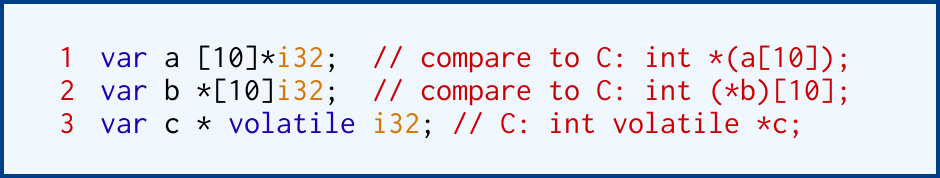
\includegraphics[scale=0.25]{gfx/types}
        \caption{Examples of variable declarations in DEF.  C allows the parentheses to be omitted in the first case, though they're provided to make precedence explicit.}
        \label{fig:types}
\end{figure}

Syntactically, DEF looks similar to C with the most apparent difference being that scopes are denoted by keywords instead of curly braces (e.g., \texttt{if} and \texttt{fi}, \texttt{do} and \texttt{od}, etc.) allowing curly braces to be repurposed for tuples.  Native types specify a bit width, so C's \texttt{int} on most systems corresponds to DEF's \texttt{i32}.  Types are also designed to read left-to-right, so the return type in a function declaration has been moved to the right using an arrow notation similar to ML-like languages or Go.  For more complicated types, fig.~\ref{fig:types} gives an example of left-to-rightness where no parentheses are needed to distinguish an array of pointers to integers (line 1) from a pointer to an array of 32-bit integers (line 2).

\begin{figure}[htbp!]
        \centering
        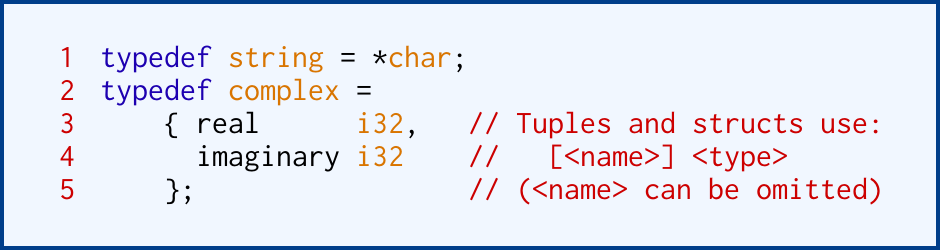
\includegraphics[scale=0.25]{gfx/typedef}
        \caption{Defining types with \texttt{typedef}.}
        \label{fig:typedef}
\end{figure}

Types are defined with the \texttt{typedef} keyword.  Figure \ref{fig:typedef} shows two examples: a C-style \texttt{string} type is defined on line 1, and a complex number struct is defined on lines 2-5.  The struct's actual definition is identical to tuple syntax, though tuples typically omit the member names.  Worthy of note is that tuples in DEF really are just anonymous structs, in keeping with the design goal of interchangeability with C.  Whereas in many languages tuples are allocated on the heap and garbage collected, in DEF they're allocated however a named struct would be in C.  Locating a struct or tuple on the heap requires explicit allocation.  Fig.~\ref{fig:window-find} provides a \texttt{window\_{}find} function declaration from the (FIXME: proper name and citation)Harris lock-free linked list in the Herlihy-Shavit book, as expressed in C (lines 2-6) and DEF (lines 9-10).  In both cases, the struct is returned by value on the stack.  A pointer, in both cases, would require explicit pointer syntax.

\begin{figure}[htbp!]
        \centering
        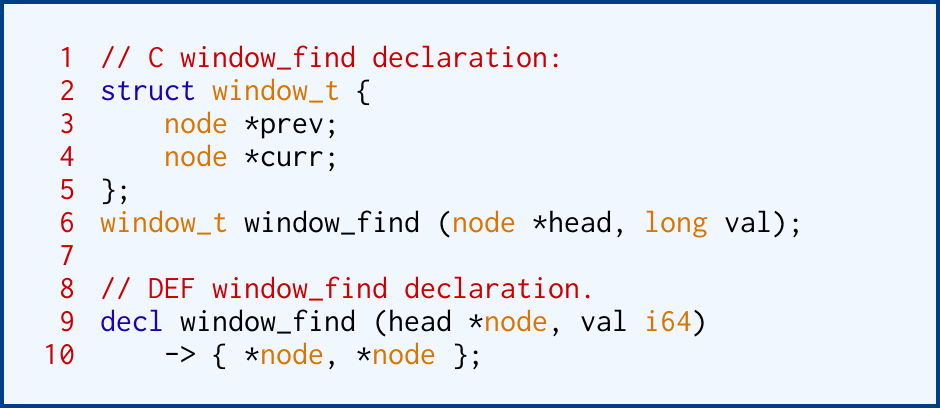
\includegraphics[scale=0.25]{gfx/window-find}
        \caption{Equivalent \texttt{window\_{}find} declarations in C and DEF.  The DEF tuple is an unnamed equivalent of C's \texttt{window\_{}t}.}
        \label{fig:window-find}
\end{figure}

\subsection{Allocation, Deallocation, and Reclamation}

DEF has no native allocator as distinct from C.  Allocating memory with \texttt{new} and deallocating it with \texttt{delete}, use \texttt{malloc} and \texttt{free}, respectively.  Since DEF's memory reclamation system is implemented using Forkscan, they implicitly use Forkscan's \texttt{malloc} and \texttt{free} wrappers, but the overhead of this indirection is undetectable in trials.  Independent of implementation, memory allocated with \texttt{new} is untracked.  Memory can be passed freely between DEF and C, and a pointer acquired in C through \texttt{malloc} can be deleted in DEF, and one acquired in DEF through \texttt{new} can be freed in C.

Moreover, \texttt{new} and \texttt{delete}, as applied to non-shared memory, are conveniences-only.  Mixing allocators or interfacing with a language with hooks to an external garbage collector is as trivial (or as complex) in DEF as it is in C because all memory is treated in exactly the same way.

The exception to this is in the use of \texttt{retire} to flag a pointer for tracking.  It's assumed that a retired node was allocated with the same allocator used by \texttt{new}.  Implementation-wise, Forkscan requires knowledge of the \texttt{free} and \texttt{malloc\_{}usable\_{}size} corresponding to the \texttt{malloc} that was used to acquire the memory.  More broadly, it's hard to see how any implementation could call the correct \texttt{free} on a retired node unless it corresponded to the known \texttt{malloc}, and this isn't especially burdensome to programmers.

A final restriction on \texttt{retire} is that it may only be called on a pointer, once.  If multiple threads retire the same memory, the behavior is undefined.  In practice, it acts like a double-free because the reclamation system may perform a double-free.  A good usage model is the thread that successfully removes a node from the concurrent data structure is the one that should retire it.  This makes its use intuitive because code looks like the familiar serial model where \texttt{retire} is replaced by \texttt{delete}.

\subsection{C Interface}

C++ is the gold-standard for interfacing with C.  As mentioned above, C header files can be included directly into C++ files, and C++ functions can be declared with C linkage.  Features like templates, classes, and member functions of structs, can't be exported to C, but anything C-like can be.  Given DEF's syntactic differences, even for features it holds in common with C, sharing DEF interface (\texttt{.defi}) files directly with C is impractical.  However, most of the function-level features have a one-to-one correspondence with C.  Therefore, the compiler is accompanied by a utility, \texttt{defghi}, for generating headers and interface files from DEF source files.

Generating headers and interface files is assisted by a formal approach to module interfaces.  A subtle distinction from C is that DEF types, functions, and globally-scoped variables are local to the module in which they appear, by default.  C's default is external visibility, and local symbols must be marked \texttt{static} by the programmer.  In contrast, DEF requires programmers to mark symbols with \texttt{export} in order to make them visible.

Since the differences are syntactic, generating header files from \texttt{defghi} is simple.  Any type, global variable, or function marked \texttt{export} has its declation unparsed into C and pretty-printed into the header.

The other direction, importing C definitions into DEF, involves recognizing headers by filename extension and passing them through a C parser.  Clang, the LLVM C compiler, collects all type definitions and function and global variable declarations, and DEF converts them into its own internal representation.  Therefore, DEF can import C headers directly as if they were native DEF.

There are two limitations to this: DEF can't import actual C functions (as opposed to function declarations), and C macros aren't resolved except where they appear in a header file itself.  In the first case, functions in header files are a planned feature that was deprioritized since they're uncommon in the C standard library, and it was reasoned that high performance programmers often do intermodule optimization, negating the value of putting them in headers.  In the second case, DEF does not yet have macros of its own, and a naive implementation of incorporating C macros might conflict with a well-designed DEF macro language.  Since C macros are simple text-substitution, integration into a language with a different syntax is another problem, altogether.
